%% LyX 1.1 created this file.  For more info, see http://www.lyx.org/.
%% Do not edit unless you really know what you are doing.
\documentclass[oneside,english]{book}
\usepackage[T1]{fontenc}
\usepackage[latin1]{inputenc}
\usepackage{babel}
\setcounter{secnumdepth}{3}
\setcounter{tocdepth}{3}
\usepackage{makeidx}
\makeindex
\usepackage{graphics}

\makeatletter

%%%%%%%%%%%%%%%%%%%%%%%%%%%%%% LyX specific LaTeX commands.
\providecommand{\LyX}{L\kern-.1667em\lower.25em\hbox{Y}\kern-.125emX\@}

\makeatother
\begin{document}

\title{Initial study}


\date{Date}


\author{Pascal Munerot}

\maketitle
\tableofcontents{}


\newpage
\part{Introduction}


\section{What is this document ?}

This document is a detailed and formal description of all the features
the Project Architect is likely to implement.\\
As the time goes by, this document will be split into sub-parts to
accomodate separate threads of discussions. \\
This document is not yet complete and will be updated whenever necessary
to match the current design issues. 


\part{Functional issues}


\section{Concept : Information visibility\index{Information visibility}}


\subsection{Domain management\index{domain management}}

There must be a domain management within the Project Architect. 


\subsubsection{Domain subscription\index{domain subscription}}

A user of the Project Architect may decide to subscribe to a domain
of the Project, that is to be notified of any incoming information
item corresponding to this domain, with respect to security issues
(Some users may not be allowed to see everything).\\


\noindent More generally, users shall be able to register many aspects
of the project life cycle (requests for features, progress, releases,
problem management). 


\section{Concept : \index{Documents}Documents}


\subsection{Document location\index{document location}}

The documents should be sheltered in only a few places. One major
goal of this project is to avoid \emph{document scattering.} Today,
the increasingly sophisticated communications allow us to exchange
information and documents in various ways. Unfortunately, this is
very bad practice because as a consequence information is not accessible
in one single place. Instead, users must search lots of places for
documents and information that quickly contradict one another (because
they have not been maintained in a controlled and centralised manner).
Thus, users have conflicting views of the same piece of information.
This turns out to be a major reason for delays, bugs and users griefs
(which may end up as the project's failure)


\subsection{Atomic documents\index{atomic documents} versus structured documents\index{structured documents}}


\subsubsection{Atomic documents}

Atomic documents are small, indivisible documents. They can be of
any type (text, drawing, xml ...) provided that they cannot be broken
in sub-parts (On the user's point of view. Obviously, there may sub-parts
as far as the storage point of view is concerned). \\
\\
Advantages over structured documents is that version control and identification
can be very tight. These documents may be included in structured documents
while still retaining their original properties. 


\subsubsection{Structured documents (also known as complex documents)}

Unlike atomic documents, structured documents can nest other documents
(atomic documents, links, ...). 


\subsection{Registered documents\index{registered documents}}

{\raggedright Registered documents are documents that are considered
sheltered and managed by the project architect. This is a generic
concept including both internal format and external format documents.
In particular, this means that the document may not be modified outside
of the Project Architect influence (Later on, we will introduce variations
on this)\\
\par}

\noindent It also includes version management, property management
(keywords, document type information, authors, intended audience,
links to other documents, security information).\\


\noindent Registered documents are given a unique identifier that
all users (using the engine of course) can refer to. It is an important
feature because this will allow to keep a tight control over a document
lifecycle (through revisions, rewrites, publications). When speaking
of a unique identifier, we mean that this identifier shall be \emph{distributed}
(considered unique over a large network, possibly the whole internet).
This identifier will contain both a technical and a user visible part.
The user visible part will be a user level shortcut to the technical
id. This may be a word, or anything. \\


\noindent This basic requirement will make it possible for users to
be notified whenever a document is modified, wherever they are.\\


\noindent An unregistered document is not considered part of the project
and therefore not handled at all by the Project Architect.


\subsubsection{External\index{external documents} and detached documents\index{detached documents}}

\noindent Some documents may be considered \emph{detached documents}
if their content is generated by another party not using the Project
Architect but is still considered part of the project under development.
An external document is a document outside the project's management
(ie. is not a part of the project, rather some external documentation).


\subsubsection{Managed document format \index{managed document format}}

Some documents formats will be known to the Project Architect or by
one of its plugins. The Project Architect will consider these document
formats as \emph{managed} because it knows how to handle them. Some
document formats may be proprietary and therefore may not be managed.
This does not mean that it will be unacceptable to register a document
using such a format.\\


\noindent Put in other words, managed data formats will be easier
to manipulate within the Project Architect and some constraints (left
on other kinds of documents) may be lifted. 


\subsubsection{Document properties\index{document properties}}

\begin{itemize}
\item Primary maintainer : This may change over time but the full list must
be kept.
\item Reviewers : It speaks itself. Again, there may be many.
\item Acceptance level : Is this document accepted by all involved parties,
it is still consistent with the current issues\ldots{}
\item Publication status : 

\begin{itemize}
\item Planned : The need for this document has been clearly expressed
\item Draft : This document is being written but is clearly at an early
stage. 
\item Released/Published : Users other than the author itself can consult
the documents. There will be refinements in the ways a document can
be published:

\begin{itemize}
\item restricted publication : Only a subset of the users will be allowed
to read the document. These users may be defined in terms of groups.
\item internally published : All the users can read the document.
\item publically published : Absolutely no restrictions are imposed on the
publication of the document
\end{itemize}
\item Revised : Documents are often revised. Several kinds of revisions
may be implemented : 

\begin{itemize}
\item full revisions : Basically, a major (if not near complete) rewrite
of the document. Previous versions of the document will be kept but
will not remain directly visible to the user. 
\item partial revisions : These revisions will include patches to the original
document. Control versionning and managed document formats will be
important here.
\end{itemize}
\end{itemize}
\item Distribution lists \index{distribution lists}: To automate distribution
of the documents
\item Security\index{Security} : Security information (see above).
\item Revision control information : This will be different from CVS style
version management for the following reasons :

\begin{itemize}
\item We want to have a fine-grained control over the kind of information
kept under control. Obviously, file level is too limited.
\item We also want to be able to move some piece of information (or document)
around without having to go into CVS like manipulations (removing
from a directory/folder, adding in another, then committing). This
should be done transparently, at least from the user point of view
(It may be done like CVS internally) : One must be able to drag and
drop items easily. 
\end{itemize}
\item Node structure : A tree depicting the document structure. XML is one
of the cool language for doing just that, but there are others. Not
all data formats will allow this (proprietary formats, monolithic
formats).
\item IsFolder : Is the document a folder (containing other documents and
folder => May be handled via node structure).
\end{itemize}

\subsubsection{Document shell\index{document shell}}

A document shell is a data structure allowing to handle modifications
to a document over time. Basically, a document can be revised (minor
modifications) or completely rewritten (major modifications). A document
shell is designed to help handle these situations by providing a \emph{shell}
(some sort of document container, sheltering a unique document, including
all the revisions, whichever way they have been implemented).


\subsection{Folder concept\index{folder}}

Create the folder concept : A folder contains everything pertaining
to some specific field/event during the project lifetime. Despite
being similar in terms of concepts, a folder shall not be confused
with a computer directory. Actually, a folder may be mapped to more
than one directory and more than one document. A document may be referenced
in several folders. It may contain links to other folder or directory.
A directory is considered some kind of dumb folder that has not much
flexibility.\\


{\raggedright A folder shall be a hook of the filesystem designed
to hide implementation details from the user. So, we must provide
a way to give a visual view of a folder in the form of a listview.
\\
\par}

{\raggedright A folder will summarize and be aware (in terms of contextual
menus) of document information (keywords, version control ...).\par}


\subsection{Information view\index{information view}}

This concept consists of implementing differents views of documents
and information, depending on the user. This may be done as automatic
reports\index{reports} (based on some sort of scripting engine).\\


\noindent Stylesheets\index{Stylesheets} may be used also (XSLT,
CSS ...).


\subsection{External documents\index{external documents}}

External documents should be allowed access by catalog. A catalog
can be loaded from the content of a given directory or new entries
may be added using a dialog (add, edit, new, delete ...)


\subsection{Views \index{Views}}

Several views should be given for a set of information and/or documents.
Atomic information should be easy to move from/to documents if the
document is an internal document (ie. It has a format that the project
architect support. Typically, this format will allow for easy information
atomicity, be a text file of some sort).


\subsection{Document generator and parser}

A system based on plugins to automatically generate documents using
always the same driver code (or syntax). \\


{\centering Also, implement a parser for analysing existing documents
in order to store them in a generic manner. This way, documents would
be better integrated in the project management lifecycle while preserving
the ability to generate any formats out of the generic version. \\
.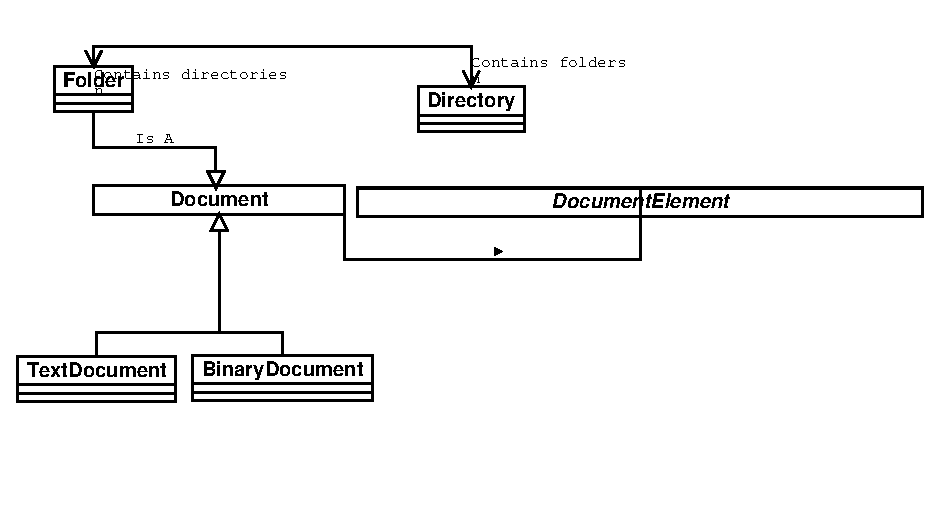
\includegraphics{analysis_documents.eps} \par}


\section{Dealing with users requests, quality assurance, development progress
and release time}


\subsection{Decision tree feature  }

A decision tree is a model depicting the process of evaluating user
requests, To be able to track down users requests, acceptance from
quality staff, development progress in a visual way. This shall be
made possible by both XML and wxWindows tree widgets (may also be
represented as listviews).\\
\\
Point of views : The decision tree will support the concept of point
of views. Several points of view may be registered before a final
decision is taken. This allows to keep tracks of all the ideas and
to decide clearly which one has been validated. Once this validation
has occurred, it is difficult for the different parties to disagree.
This will increase the overall quality and efficiency. \\
\\
Decision / point of view revisions : Point of views and decision may
be revised. If a validated decision is revised, then the new version
becomes the official decision. 


\part{Technical issues}


\section{Architecture issues - Living in a distributed world}

This part gets a lot more technical than the first part. Here, we
will introduce ideas that will serve as ground for the distributed
architect used for implementing the Project Architect.


\subsection{Retargettable client applications}

The Project Architect is a client-server (n-tier) application. Access
to a project repository shall be allowed from different places and
different setups. Basically, an ideal situation would be the following
:

\begin{itemize}
\item Client applications : 

\begin{itemize}
\item A client middleware module will serve the purpose of converting and
transporting the data from the client to the server. This middleware
is included in the client but is also highly tied to the server. The
reason for which this module is in between the client is that its
role is mainly to convert data in the client space to data in a serialized
form. The serialized data is then sent to the server, which executes
the query and returns the result in a serialized form. The middleware
will then deserialize the data back to something usable in the client
address space. Something important to understand is that this middleware
is not a process separate to the client. It is part of the client
itself (and in particular lies in the same address space). 
\item User interfaces : 

\begin{itemize}
\item A native GUI application, in the standalone style but naturally distributed 
\item A web interface (to allow use from a browser), with a Java front -
end
\end{itemize}
\end{itemize}
\item Server applications : 

\begin{itemize}
\item Engine : In charge of routing everything to the sub-processes, these
sub-processes being in charge of some specific details. Scalability,
load-balancing and fail-over issues should also be considered. Server
processes typically handle the hard work of organizing, storing, retrieving
and processing the information system. It comprises an engine organized
as a single process. \\
\\
This process may be cloned in order to achieve load-balancing. The
engine implements a full server side middleware (very similar to the
client side middleware but the other way round). This module will
(de)serialize data and convert it to fit the server process's address
space. Therefore, the middleware is fully part of the server process.
\\
\\
A server middleware module serving the purpose of deserializing the
data. Like the client middleware, it is not a separate process. In
the case of the server side, this means that it is part of the engine
process. 
\end{itemize}
\end{itemize}
{\centering \resizebox*{0.3\textwidth}{0.3\textheight}{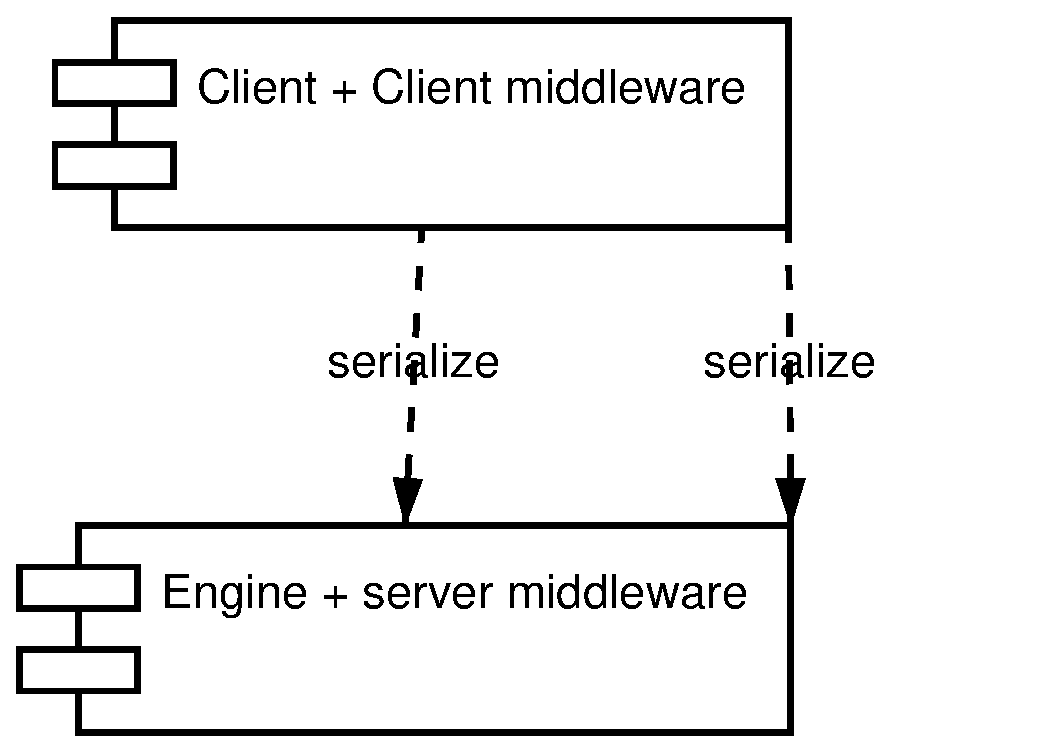
\includegraphics{architecture_overview.eps}} \par}


\subsection{Repository structure }

The repository shall be organized in order to be able to deal with
requests from many places. This shall lead to the following structure:

\begin{itemize}
\item The organisation repository : This is a repository shared by all the
organisation and therefore all the users, wherever they are. This
approach will not be implemented at first because of development priority.
\item The project repository : This will store all information relevant
to a project (we mean everything).
\end{itemize}
It is not yet decided whether the repository shall be organised as
a main directory or as a binary b-tree style binary file. They are
big issues since both approaches have drawbacks and advantages :

\begin{itemize}
\item Binary b-tree files

\begin{itemize}
\item The information is stored in one place, so backups are facilitated.
\item You can easily store any kind of information, ranging from small information
items to big documents
\item users cannot easily tinker with the content and may not break it
\item Unfortunately, b-trees must be reorganized often to keep them away
from corruption
\end{itemize}
\item Directories

\begin{itemize}
\item Information is stored in many places
\item Unfortunately, directories cannot easily store small information items.
This can be dealt with by using files for storing smaller items.
\end{itemize}
\item Full database systems : 

\begin{itemize}
\item A lot of power in terms of storage and queries. 
\item Data visibility is good
\item Still, DBMS are limited in their flexibility. New concepts cannot
be easily added without sacrifing their power. Constantly changing
data structures or data structures implemented by the user are not
easily fitted in a database system. 
\item It adds more administration constraints to the whole system (Installation
as a server process, another dependency for the project using it).
\end{itemize}
\item Necessary technical modules
\end{itemize}
This part is an attempt to list out the modules necessary for the
implementation of the project This tables contains several entries.
One for the module description, another for the modules that may use
it as a supplier of service. 

{\raggedright Those modules adopt an organisation based upon layers
in order to achieve modularity, portability and reusability of code.\par}


\section{Implementation model}


\subsection{Layers list and description}

\begin{itemize}
\item The \emph{\char`\"{}external layer\char`\"{}} : It the C++ library
used to implement the framework. It must be a portable library (wxWindows?).
It does not explicitly belong to the project but is a supplier for
the project. \emph{WxWindows} has a lot of nice features. A graph
module and a great concern for portability are among them. A related
project, \emph{wxStudio} (an IDE for developping \emph{wxWindows}
applications) is under development and is not yet usable (unfortunately).
\item The \emph{\char`\"{}framework layer\char`\"{}} implements a low-level
behavior. This could be a common framework for several projects. It
has low level and very generic services. It is supposed to be a supplier
for concrete implementation of the project. Portability problems should
be solved in this layer. Therefore, this layer shall give a fully
portable interface (ie. It must provide a consistent set of API for
higher level layers.
\item The \emph{\char`\"{}services layer\char`\"{}} is a medium level one.
Less generic and more to the point services. Here we implement the
core of the project. This layer may be split in several parent and
sibling layers in a client/provider fashion. Services must be well
isolated and fulfill a small set of services. Plugs-in can be hooked
here using the API provided by these layers.
\item The \emph{\char`\"{}application layer\char`\"{}} is the actual presentation
layer (GUI) for the project. It may be split across different applications
linked together by a common interface. It allows data entry, processing,
reporting, everything the project provides to the user ...
\end{itemize}
\vspace{0cm}
{\centering \resizebox*{0.3\textwidth}{0.3\textheight}{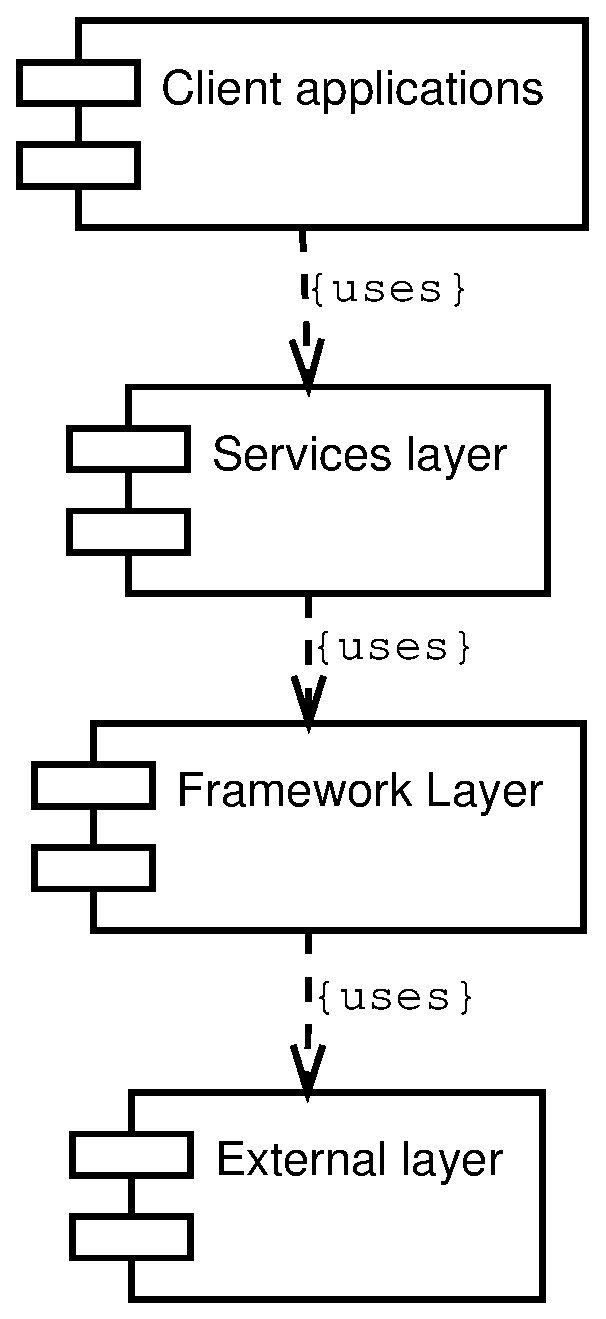
\includegraphics{layers.eps}} \par}
\vspace{0cm}


\subsection{Modules list }

See the modules list document

Naming conventions (not well defined at the moment)

The naming convention is there to facilitate comprehension and maintenance
of the source code. It is as follows :

A prefix : pa : To give the idea of a namespace (C++ namespace instead)

The name of the generic services fulfilled by the module : data, server,
parser, storage, index

The name of a more specific service : xml .... 

Instance id for the module, necessary when several modules are close
in their behaviour and role.

Version number : major and minor. Better implemented at runtime than
at compile time because of the problem of name updating.


\subsection{Plugin implementation}

Plugins will be implemented as threads so that they can be pinged
whenever necessary. Also, this will make them more flexible. The plugin
implementation naturally belongs to the Framework layer. \\


{\raggedright In order to ease creation of plugins, a C API and bindings
for Perl, Python (and Tcl?) will be provided.\\
\par}

\printindex{}
\end{document}
